\documentclass[14 pt]{extarticle}

	\usepackage[frenchb]{babel}
	\usepackage[utf8]{inputenc}  
	\usepackage[T1]{fontenc}
	\usepackage{amssymb}
	\usepackage[mathscr]{euscript}
	\usepackage{stmaryrd}
	\usepackage{amsmath}
	\usepackage{tikz}
	\usepackage[all,cmtip]{xy}
	\usepackage{amsthm}
	\usepackage{varioref}
	\usepackage{geometry}
	\geometry{a4paper}
	\usepackage{lmodern}
	\usepackage{hyperref}
	\usepackage{array}
	 \usepackage{fancyhdr}
	 \usepackage{float}
\renewcommand{\theenumi}{\alph{enumi})}
	\pagestyle{fancy}
	\theoremstyle{plain}
	\fancyfoot[C]{} 
	\fancyhead[L]{Devoir maison}
	\fancyhead[R]{pour le 7 novembre 2022}\geometry{
 a4paper,
 total={170mm,257mm},
 left=20mm,
 top=20mm,
 }
	
	
	\title{DM}
	\date{}
	\begin{document}

\begin{center}{\Large Devoir Maison}\\ 
 \end{center}
 \subsection*{Exercice 1 }
 
Pour les calculs suivants, numérotez les opérations, puis effectuez-les étape par étape. \begin{enumerate}
\item $2+3\times 5 - 4$
\item $6\times 4 \div 3 \times 2$
\item $30 \div (3 + 4\times 5 \div 2+2)$
\item $2 + 3 - 5 + 4 - 2 \times (4 - 2 + 2) \div 2$
\item $(4 - (3\times 6 \div 9)) \times (2 + (3\times 4 \div 2+2))\div 2 + 3$
\end{enumerate}
 
 \subsection*{Exercice 2 }
Factorisez les expressions suivantes, puis calculez les : 
\begin{enumerate}
\item $7 \times 23 + 93 \times 23$
\item $ 291 \times 41 - 91 \times 41$
\item $ 324 \times 27 - 27 \times 24$
\item $ 123 \times 101 + 99 \times 123$
\end{enumerate}
\subsection*{Exercice 3} 
Rappelez les définitions des objets suivants : \begin{enumerate}
\item le milieu d'un segment.
\item la médiatrice d'un segment. 
\end{enumerate}
Recopiez et complétez : 
\begin{enumerate}
\item Si deux droites sont symétriques par rapport à un point, alors \ldots
\item Si $A$ et $B$ sont symétriques par rapport à $(d)$, 
alors $(d)$ est la \ldots du segment $[AB]$. 
\end{enumerate}

 \subsection*{Exercice 4}
 \begin{enumerate}
 \item  Tracez un triangle équilatéral $ABC$ de côté $3$ cm. 
\item Tracez le symétrique $A_1B_1C_1$ du triangle $ABC$ par rapport au point $A$.  
\item Tracez le symétrique $A_2B_2C_2$ du triangle $ABC$ par rapport au point $B$.  
\item Tracez le symétrique $A_3B_3C_3$ du triangle $ABC$ par rapport au point $C$.  
\item Sur la figure obtenue, tracez tous les axes de symétrie. 
\item Y a-t-il un centre de symétrie ? 
\end{enumerate}
 \subsection*{Exercice 5}
 
Calculez la surface de la figure suivante, où tous les triangles sont des rectangles isocèles identiques. Expliquez votre raisonnement.

\begin{figure}[H]
\center
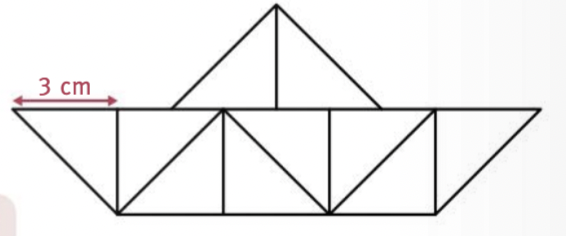
\includegraphics[scale=1]{Bateau}\end{figure}

\subsection*{Exercice 6}

\begin{enumerate}
\item Tracez un triangle $ABC$ quelconque. 
\item Tracez le point $D$, symétrique de $B$ par rapport à $A$. 
\item Tracez le point $E$, symétrique de $C$ par rapport à $A$. 
\item Tracez le point $F$, symétrique de $D$ par rapport à $E$. 
\item Tracez le point $G$, symétrique de $B$ par rapport à $C$. \\ \\Raisonnement à partir des propriétés du cours : 
\item On note $F'$ le symétrique de $F$ par rapport à $A$. \textbf{Montrez que} $F'$ appartient à $(BC)$.
\item \textbf{Montrez que} $C$ est le milieu de $[BF']$. 
\item Déduisez-en que $F'$ et $G$ sont confondus (= sont le même point.)

\end{enumerate}



 	\end{document}
